\chapter{Deployment Design}
      In this high-level deployment diagram, we show the technologies used for each component of the system. The client will use HTML, CSS, and JS, and will be run on the user’s machine. This will communicated with the server, which will be built with Nodejs and will run on a Unix system. These components will use a Postgres Database in order to store all of the information of the system (user results, assignments, etc.). The database will be on the same machine as the server.
                        \begin{figure}[H]
            \centerline{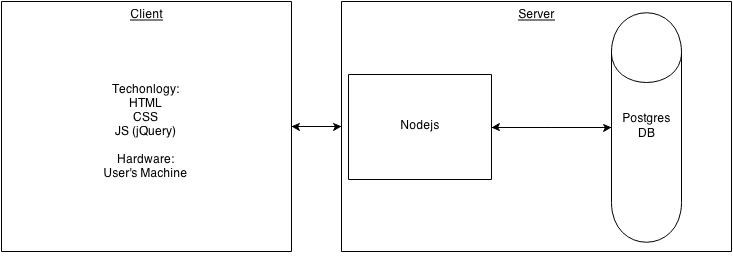
\includegraphics[height=3cm, width=10cm]{Deployment.jpg}}
            \caption{Deployment Diagram}
    \end{figure}
    
\chapter{Modular Design}
In this more detailed architecture design you can see the different modules in both the client and server sides.  The Client is made up of the Drawing Widget, Report Formatter, and Serializer while the Server is made up of the Deserializer, Dispatcher, Validator, DB Accessor and the DB.  The Drawing Widget contains everything needed for the user, author or student, to draw out either the question, answer or solution to a question that is displayed on the screen.  The Report Formatter is only used by the instructor user and takes the information that it receives from the database to compile a report on the students for the instructor to view.  The Serializer, is used for packaging and submitting the question and answer from the user to the server through http sending as a JSON.  The Deserializer is used to take what was sent from the server and undo the serialization that was used when sending information to the server.  On the Server side, the Dispatcher takes the information from the Server and packages the information to be sent to the client side of the system.  The Validator is used when a student submits an answer to a question to check the answer for correctness, and generate feedback to the student.  The DB Accessor is responsible for handling all of the requests made to send or receive information from the database.  Finally the DB is the database that contains the question bank, the student responses and assignments.    
 
                        \begin{figure}[H]
            \centerline{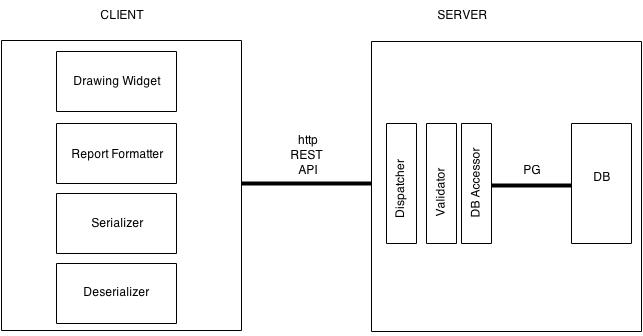
\includegraphics[height=5cm, width=10cm]{Modular.jpg}}
            \caption{Modular Diagram}
    \end{figure}
    
    \chapter{Client}
This is the diagram for the Client module. The following are the methods contained in it. openAssignment() is used by both students and instructors to open an assignment. It calls sendPageRequest() and renderPage() to render the page. createAssignment() is used by an instructor to create an assignment. openQuestion() is used by all three users, the authors, the instructors, and the students to open a question. It uses the render methods to render the page. The createQuestion() method is used by an author to create a question. drawDiagram() is used by both authors when creating the diagram and students when answering it. It uses the methods in DrawingWidget. placeEntity() to place the entities in the diagram, placeRelation() to place the relations in the diagram, and addText() to add text to the diagram. submitAnswer() is used to submit a diagram and calls sendToSerial() in DrawingWidget which uses the Serializer methods createSerialJSON() to convert the diagram into a JSON format, and sendJSON() to send this JSON to the server. openReport() is used by an instructor to view the student reports. The methods in ReportFormatter are used, collectStudentReports() retrieves the reports from the server, formatReports() formats the reports to be viewed, and render() renders the webpage.  When diagrams are sent back to the client from the server they go through the Deserializer which calls the methods, recieveJSON() when the JSON is passed back from the server and then unpackSerialJSON() to unpack the JSON back into a diagram.
  
                        \begin{figure}[H]
            \centerline{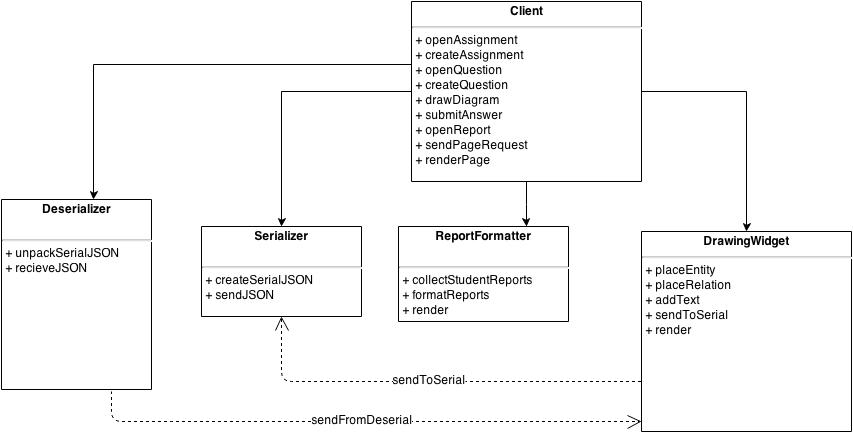
\includegraphics[height=5cm, width=10cm]{Client.jpg}}
            \caption{Client Diagram}
    \end{figure}
    
    \chapter{Server}
The server plays a huge role in our system, it is in charge in keeping connection with the Client and the database. The Dispatcher will process the question submitted by the user and request its validation with the validator. Then, the validator checks whether the question submitted by the student is actually right or not, by going to the database accessor. Moreover, when validator check if a question is right or not, it sends a customized feedback for that particular question.
The server also is able to update a particular question in the database that has been saved by the author. 

                        \begin{figure}[H]
            \centerline{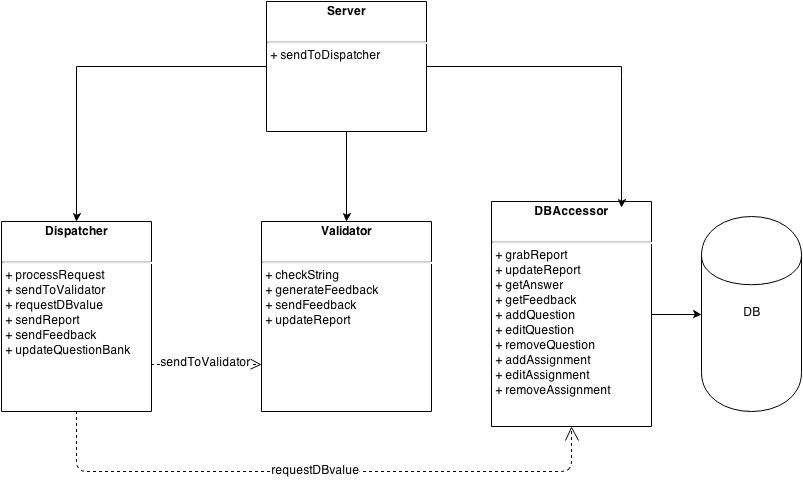
\includegraphics[height=4cm, width=10cm]{Server.jpg}}
            \caption{Server Diagram}
    \end{figure}
    